\scanpage{405}
% The handwriting is inverted relative to the archive number.
% One continuous oblique cancellation crosses the diagrams marked below.
\deleted{\diagram{\begin{tikzcd}[ampersand replacement=\&,column sep=small]
U \arrow[d,"W"'] \& \overset{W}{\subset} \& \bar U \arrow[d,"W"] \& \subset \& X \arrow[d,no head] \& \supset \& Y \arrow[d,Rightarrow]\\
U' \& \underset{W}{\subset} \& \bar U' \& \subset \& X' \& \supset \& Y
\end{tikzcd}}}
\[
\bar U\cap Y=\dot Y
\]
\margin{\uline{p.~124,125} / p.~\unsure{264|254}\\ à faire \unsure{rajout}\\ \deleted{$\unsure{X}_{0}$}}

\deleted{\diagram{\begin{tikzcd}[ampersand replacement=\&,row sep=small,column sep=small]
\&Y\arrow[rrdd]\arrow[dd,no head]\&\&\\
\dot Y\arrow[ur]\arrow[dr,thick]\arrow[dddd,no head]\&\&\&\\
\&\bar U\arrow[rr]\arrow[dddd]\&\&X\arrow[dddd,no head,"W"]\\
\&\&\&\\
\&Y'\arrow[rrdd]\&\&\\
\dot Y\arrow[ur]\arrow[dr,thick]\&\&\&\\
\&\bar U'\arrow[rr]\&\&X'
\end{tikzcd}}}
\[
X_1
\]
\deleted{\diagram{\begin{tikzcd}[ampersand replacement=\&,row sep=tiny,column sep=small]
\&\&X_1\&\&\\
\displaystyle\int\&X_0\arrow[ur]\arrow[dr]\&{}\arrow[rr,very thick]\&\&X\\
\&\&X_2\&\&
\end{tikzcd}}}
\diagram{\begin{tikzcd}[ampersand replacement=\&,row sep=small,column sep=small]
\&X\arrow[dr,no head]\&\\
S\arrow[ur,no head,"\mathrm{Cof}_{W}"]\arrow[dr,no head,"\mathrm{cof}_{W}"']\arrow[dd]\&\&\bullet\\
\&Y\arrow[ur,no head]\&\\
S'\&\&\mathrm{Fib}_{W}\cap W
\end{tikzcd}}
\deleted{\diagram{\begin{tikzcd}[ampersand replacement=\&]
X_{0y}\arrow[r,no head]\arrow[d]\&X_{1y}\\
e\&
\end{tikzcd}}}
\deleted{\diagram{\begin{tikzcd}[ampersand replacement=\&,column sep=small]
Z\arrow[rr,very thick]\arrow[dr,thick]\&\&Z\arrow[dr,dashed]\&\\
\&e\arrow[rr,dash dot]\&\&\unsure{\circ|0}
\end{tikzcd}}}

\figure{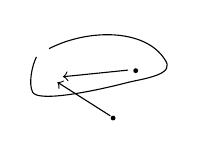
\begin{tikzpicture}[scale=.7]
\draw (-1.08,.43) .. controls (-.38,.79) and (.66,.8) .. (1.02,.23) .. controls (1.21,-.03) and (.72,-.1) .. (.36,-.18) .. controls (-.25,-.34) and (-1.28,-.55) .. (-1.38,-.36) .. controls (-1.46,-.21) and (-1.39,.13) .. (-1.31,.28);
\fill (.49,.03) circle (1.25pt); \fill (.08,-.83) circle (1.25pt);
\draw[->] (.35,.04)--(-.83,-.08); \draw[->] (.03,-.79)--(-.93,-.18);
\end{tikzpicture}}

\deleted{\diagram{\begin{tikzcd}[ampersand replacement=\&,row sep=small,column sep=small]
\&X_{\unsure{1}}\arrow[dr]\arrow[ddd,no head,"W"']\&\\
X_0\arrow[ur,"\alpha_1"]\arrow[dr,"\alpha_2"']\arrow[ddd,"\mathrm{id}"']\&\&\unsure{\mathscr X|\mathcal X}\arrow[ddd,"\mathrm{id}"]\\
\&X_2\arrow[ur]\arrow[ddd,"W"]\&\\
\&\overset{\unsure{+|\downarrow}}{X'_1}\arrow[dr,dash pattern=on 2pt off 1pt on 2pt off 1pt on 2pt off 1pt on 120pt off 0pt]\&\\
X_0\arrow[ur,no head,"\alpha'_1"]\arrow[dr,"\alpha'_2"']\&\&\mathscr X\\
\&X'_2\arrow[ur]\&
\end{tikzcd}}}
% archive sheet number: 404
